Předkládaná práce se zabývá základním typem magneto-optického experimentu, který je schematicky znázorněn na obr. \ref{fig:uvodni-diagram}.
Tato kapitola shrnuje některé fyzikální modely a jevy důležité pro jeho popis.

\begin{figure}[htbp]
    \centering
    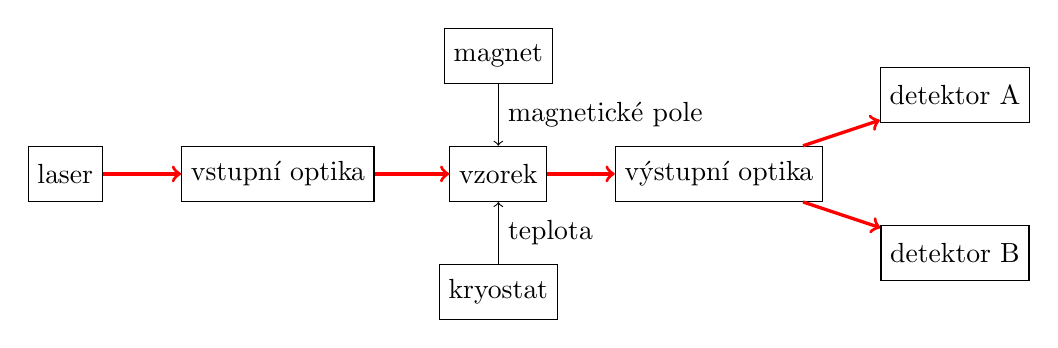
\begin{tikzpicture}[lase/.style={color=red, very thick}]

\begin{scope}[every node/.style={draw,shape=rectangle,minimum size=0.7cm}]
    \path (0,0) node (laser) {laser};
    \path (laser) +(2.7,0) node (inopt) {vstupní optika};
    \path (inopt) +(2.8,0) node (vzorek) {vzorek};
    \path (vzorek) +(0,1.5) node (magnet) {magnet};
    \path (vzorek) +(0,-1.5) node (kryostat) {kryostat};
    \path (vzorek) +(2.8,0) node (outopt) {výstupní optika};
    \path (outopt) +(3,1) node (detA) {detektor A};
    \path (outopt) +(3,-1) node (detB) {detektor B};
\end{scope}


\draw[->,lase] (laser) -- (inopt);
\draw[->,lase] (inopt) -- (vzorek);
\draw[->,lase] (vzorek) -- (outopt);
\draw[->,lase] (outopt) -- (detA);
\draw[->,lase] (outopt) -- (detB);


\draw[->] (magnet) -- node[anchor=west] {magnetické pole} (vzorek);
\draw[->] (kryostat) -- node[anchor=west] {teplota} (vzorek);

\end{tikzpicture}

    \caption{Schéma typického magneto-optického experimentu. 
    Laserový svazek je vhodně upraven vstupní optikou, dále dopadá na vzorek, kterým je propuštěn/odražen, nakonec je upraven výstupní optikou (a případně rozdělen do více ramen) a je detekována jeho intenzita. 
    Vzorek je umístěn v kryostatu a mezi rameny elektromagnetu, takže během experimentu mu vnucujeme libovolnou teplotu a magnetické pole.}
    \label{fig:uvodni-diagram}
\end{figure}


\paragraph{Světlo}
popisujeme Maxwellovými rovnicemi.
Je monochromatické na kruhové frekvenci $\omega$.
K popisu polarizačního stavu používáme Jonesovy a Stokesovy vektory.
Všechny optické prvky jsou lineární a nedepolarizační, takže je popisujeme Jonesovou a Muellerovou maticí\cite{gilReviewMuellerMatrix2014}.
Neúnavně využíváme grafické znázornění Muellerových matic metodou zobrazování Poincarého sféry\footnote{angl. Poincaré sphere mapping} (tzv. \emph{charakteristických elipsoidů})\cite{gilReviewMuellerMatrix2014,ossikovskiPoincareSphereMapping2013}.
O interakci světla s látkou předpokládáme, že probíhá pouze skrze vektory elektrické polarizace $\vec{P}$, magnetizace $\vec{M}$ a proudové hustoty $\vec{j}$. 

Odezva materiálů je lineární a lokální, a je obecně anizotropní. 
Uvnitř tenkých\footnote{Tak tenkých, že je nutné považovat vícenásobné odrazy za navzájem koherentní.} vzorků je nutné řešit Maxwellovy rovnice, výstupem výpočtu je opět Jonesova a Muellerova matice.
Výpočet je proveden v rámci Berremanova formalismu\cite{berremanOpticsStratifiedAnisotropic1972} $4\times 4$ přenosových matic pro anizotropní vrstevnaté prostředí, který je ekvivalentní Yehově $4\times 4$ maticové algebře\cite{yehElectromagneticPropagationBirefringent1979}, ale netrpí některými technickými nedostatky\cite{xuOpticalDegeneraciesAnisotropic2000,wuSingularitiesMatrixFormalisms2018,garibelloSingularityYehTransfer2020,bertrandGeneralAnalyticalTreatment2001}.
        
\paragraph{Magnetické látky} mají dodatečný magnetický termodynamický stupeň volnosti (parametr uspořádání).
Magneto-optickou aktivitu modelujeme jako závislost efektivní permitivity $\varepsilon$ na magnetickém stupni volnosti.

U feromagnetů je to celková magnetizace $\vec{M}$. 
Feromagnety reagují na vnější magnetické pole změnou rovnovážné magnetizace, která je daná magnetickou volnou energií (magnetickou anizotropií).
Pro tenké magnetické filmy používáme Stonerův-Wohlfarthův model\cite{stonerMechanismMagneticHysteresis1991} pro materiál v jedno-doménovém stavu; předpokládáme konstantní velikost magnetizace a nulový průmět do normály vzorku (magnetizace je tzv. \emph{in-plane}).
Efektivní permitivita je funkcí $\vec{M}$ a je rozvedena do mocninné řady, jejíž koeficienty tvoří složky lineárního $\mathbb{K}$ a kvadratického $\mathbb{G}$ magneto-optického tenzoru\cite{visnovskyOpticsMagneticMultilayers2018}.

U kolineárního antiferomagnetu FeRh (viz kap. \ref{chap:vzorek-ferh}) je magnetickým stupněm volnosti magnetizace podmřížky (Néelův vektor\todo{pravda?} $\vec{L}$)\cite{saidlUltrarychlaLaserovaSpektroskopie2018}.
Podobně jako u feromagnetů je $\varepsilon$ funkcí $\vec{L}$, až na to, že lineární člen je zakázán symetrií\footnote{Podmřížky s opačnou magnetizací jsou ekvivalentní, což obecně neplatí u všech antiferomagnetů.}.
